\documentclass[12pt, a4paper]{report}

\usepackage{listings}           \usepackage{graphicx}
\usepackage{geometry}           \usepackage{etoolbox}
\usepackage{parskip}            \usepackage{caption}
\usepackage{subcaption}         \usepackage{hyperref}
\usepackage{lmodern}            \usepackage{minted}
\usepackage{array}              \usepackage{listings}
\usepackage{xcolor}             \usepackage{pdfpages}
\usepackage[section]{placeins}
\usepackage[utf8]{inputenc}
\usepackage[T1]{fontenc}
\lstset { %
    language = C++,
    backgroundcolor=\color{black!5}, % set background colour
    basicstyle=\footnotesize,% basic font setting
}
\definecolor{LightGray}{gray}{0.9}
\definecolor{Arsenic}{rgb}{0.1, 0.1, 0.1}
%=================================================================
\makeatletter
% \patchcmd{<cmd>}{<search>}{<replace>}{<success>}{<failure>}
% --- Patch \chapter
\patchcmd{\@makechapterhead}{50\p@}{\chapheadtopskip}{}{}% Space from top of page to CHAPTER X
\patchcmd{\@makechapterhead}{20\p@}{\chapheadsep}{}{}% Space between CHAPTER X and CHAPTER TITLE
\patchcmd{\@makechapterhead}{40\p@}{\chapheadbelowskip}{}{}% Space between CHAPTER TITLE and text
% --- Patch \chapter*
\patchcmd{\@makeschapterhead}{50\p@}{\chapheadtopskip}{}{}% Space from top of page to CHAPTER TITLE
\patchcmd{\@makeschapterhead}{40\p@}{\chapheadbelowskip}{}{}% SPace between CHAPTER TITLE and text
\makeatother
% Set new lengths
\newlength{\chapheadtopskip}\setlength{\chapheadtopskip}{0pt}
\newlength{\chapheadsep}\setlength{\chapheadsep}{10pt}
\newlength{\chapheadbelowskip}\setlength{\chapheadbelowskip}{10pt}

\newgeometry{
    top=2cm,
    bottom=2cm,
    outer=1.5cm,
    inner=1.5cm,
}
%=================================================================
\title{ICS2210 CourseWork}
\author{Keith Farrugia 11104L}
\date{March 2024}

\begin{document}

\maketitle

\tableofcontents

\chapter{Statement of Completion and Plagiarism Declaration}

\begin{center}
\begin{tabular}{ | p{0.6\textwidth} | c | } 
    \hline
    \textbf{Item} & \textbf{Completed (Yes/No/Partial)} \\ 
    \hline
    Created first array of integers & Yes \\ 
    \hline
    Knuth shuffle & Yes \\ 
    \hline
    Inserted in AVL tree & Yes \\ 
    \hline
    AVL tree insertion statistics & Yes \\ 
    \hline
    Inserted in Red-Black tree & Yes \\ 
    \hline
    Red-Black tree insertion statistics & Yes \\ 
    \hline
    Inserted in Skip List & Yes \\ 
    \hline
    Skip List insertion statistics & Yes \\ 
    \hline
    A discussion comparing data structures & Yes \\ 
    \hline
\end{tabular}
\end{center}



\includepdf[pages={1}]{ICS2210 Plagiarism From - Keith Farrugia 11104L.pdf}

\chapter{Introduction}
Language: C++

The following report will serve to explain the implementation of the required 3 data structures, these being an AVL-Tree, a Black-Red-Tree and a Skip List. The report will also highlight how the required statistics are collected and analyse the results. 

In terms of the code repository's organisation, each data structure can be located in its respective folder. In each of the 3 cases, it can be seen that the implementation is usually split into more than just a single C++ and Header file. This was done for easier readability, especially for larger functions.

The repository also compiles 2 binaries one for the 5000 array insert using Knuth's shuffle and the other for the 1000 random number insertion with possible non-unique insertations.

Another point worth mentioning is that many of the comments in the main repository are committed in the code snippets listed in this report. This is to lessen the amount of text and help with clarity.

\chapter{Knuth Shuffle}
The implementation of the Knuth Shuffle is relatively simple. The function traverses the array while swapping each value at each position with another value in the array between 0 and "i" (inclusive).
\begin{minted}[frame=lines,framesep=2mm,baselinestretch=1.2,bgcolor=LightGray,
fontsize=\footnotesize,linenos]{c++}
void swap(int* array, int index_1, int index_2){
    int temp = array[index_1];
    array[index_1] = array[index_2];
    array[index_2] = temp;
}

void knuthShuffle(int* array, int size) {
    for (int i = size - 1; i > 0; --i) {
        int j = std::rand() % (i + 1);
        swap(array, i, j);        
    }
}
\end{minted}
To shuffle an array of 5000 integers the implementation below was used. Here the array "randomNumbers" was generated having incrementing values from 1 - 5000. Knuths shuffle was used to shuffle the array. The two outputs can be seen in the output of the executable
"5000\_insert".

\begin{minted}[frame=lines,framesep=2mm,baselinestretch=1.2,bgcolor=LightGray,
fontsize=\footnotesize,linenos,breaklines=true]{c++}
const int arraySize = 5000;
int randomNumbers[arraySize];

for (int i = 0; i < arraySize; ++i) {
    randomNumbers[i] = i + 1;
}

printf("\n================================ Before Shuffle ================================\n");
printArray(randomNumbers, arraySize);

knuthShuffle(randomNumbers, arraySize);

printf("\n================================ After Shuffle ================================\n");
printArray(randomNumbers, arraySize);
\end{minted}

\chapter{AVL Tree}
\section{Utility Functions}

The AVL tree is implemented through nodes each node holding a value, the height at that node, and then 2 pointers each pointing to the right or left node/subtree respectively.

\begin{minted}[frame=lines,framesep=2mm,baselinestretch=1.2,bgcolor=LightGray,
fontsize=\footnotesize,linenos,breaklines=true]{c++}
typedef struct node_t {
    int value;    
    int height; 
    AVLTree::node_t *left;  
    AVLTree::node_t *right;

    node_t(int val) : value(val), left(nullptr), right(nullptr), height(1) {}
}node_t;
\end{minted}
The following are other utility functions, getNodeHeight returns the height of a node from its height variable. This is more for reliability as it returns 0 if the node is a null leaf instead of causing a segmentation fault. The other function getBalance() returns the balancing factor of a node by calculating the difference between the left and right subtree heights.
\begin{minted}[frame=lines,framesep=2mm,baselinestretch=1.2,bgcolor=LightGray,
fontsize=\footnotesize,linenos,breaklines=true]{c++}
int AVLTree::getNodeHeight(AVLTree::node_t* node){
    if(node != nullptr){return node->height;}
    return 0;
}
int AVLTree::getBalance(AVLTree::node_t* node) {
    if (node == nullptr) return 0;
    return getNodeHeight(node->left) - getNodeHeight(node->right);
}
\end{minted}

The functions below are also utility functions and are mostly of use in statistics functions later on. The getHeight() function makes use of the fact that nodes hold the height of the subtree with them as the root, hence it returns the height of the root node. The two other functions work together to calculate the number of leaves the tree has by incrementing a counter the moment a leaf with no children is found.

\begin{minted}[frame=lines,framesep=2mm,baselinestretch=1.2,bgcolor=LightGray,
fontsize=\footnotesize,linenos,breaklines=true]{c++}
int AVLTree::getHeight() {
    return rootNode->height;
}


int AVLTree::getNumLeaves() {
    return getNumLeavesUtil(rootNode);
}

int AVLTree::getNumLeavesUtil(node_t* node) {
    if (node == nullptr)
        return 0;
    
    if (node->left == nullptr && node->right == nullptr)
        return 1;
    
    return getNumLeavesUtil(node->left) + getNumLeavesUtil(node->right);
}
\end{minted}

The code snippet below is worth noting as it is vital for the statistics gathering as well as being repeated in all 3 data structures. The variables below are used to keep track of the number of steps and rotations/promotions being taken during the insert sequence. The function updateStatistics() makes sure to reset the temporary variables after they are pushed into the record. The function is usually called at the end of the insert function. It is worth noting that although non-unique (repeating) values are ignored, their related statistics are still stored in the record as a certain amount of steps are still usually taken and it is important to take into account how these affect performance.

These will mostly referenced in a later section as since the implementation is almost identical there is no need for the code snippets to be restated.
\begin{minted}[frame=lines,framesep=2mm,baselinestretch=1.2,bgcolor=LightGray,
fontsize=\footnotesize,linenos,breaklines=true]{c++}
// ------------------------- Statistics
void updateStatistics();
// -------------- Steps
int temporarySteps;
std::vector<int> stepsRecord;
// -------------- Rotations
int temporaryRotations;
std::vector<int> rotationsRecord;

// Inside the AVLStatistics.cpp file

void AVLTree::updateStatistics(){

    stepsRecord.push_back(temporarySteps);
    rotationsRecord.push_back(temporaryRotations);
    
    temporarySteps = 0;
    temporaryRotations = 0;
}
\end{minted}

\section{Rotation Functions}
The rotation functions are isolated into their own separate .cpp files for both Avl and Black Red Trees. The rotations for the AVL trees are fairly straightforward, involving a simple switch of the pointers for the nodes. The height of each subtree is recalculated though, for them to be updated since certain subtrees have their roots changed. The right-left rotations and the left-right rotations are also implemented here in order for the functions using them, later on, to be more readable. Note that in the code implementation, there are comments above each function that make use of diagrams to better explain what the result of the rotations is.
\begin{minted}[frame=lines,framesep=2mm,baselinestretch=1.2,bgcolor=LightGray,
fontsize=\footnotesize,linenos,breaklines=true]{c++}
AVLTree::node_t* AVLTree::rightRotate(AVLTree::node_t *y){  
    AVLTree::node_t *x = y->left;  
    AVLTree::node_t *z = x->right;  
  
    // Perform rotation  
    x->right = y;  y->left = z;  
  
    // Updated Heights  =      MAX     (Height of Left SubTree   ,  Height of Right SubTree)        +  Current Node
    y->height           =      std::max(getNodeHeight(y->left)   ,  getNodeHeight(y->right))        +       1;  
    x->height           =      std::max(getNodeHeight(x->left)   ,  getNodeHeight(x->right))        +       1;  
  
    // Return new root  
    return x;  
}
AVLTree::node_t* AVLTree::leftRotate(AVLTree::node_t *y){  
    AVLTree::node_t *x = y->right;  
    AVLTree::node_t *z = x->left;  
  
    // Perform rotation  
    x->left = y;  
    y->right = z;  
  
    // Updated Heights  =      MAX     (Height of Left SubTree   ,  Height of Right SubTree)        +  Current Node
    y->height           =      std::max(getNodeHeight(y->left)   ,  getNodeHeight(y->right))        +       1;  
    x->height           =      std::max(getNodeHeight(x->left)   ,  getNodeHeight(x->right))        +       1;    
  
    // Return new root  
    return x;  
}  
AVLTree::node_t* AVLTree::leftRightRotate(AVLTree::node_t* y) {
    y->left = leftRotate(y->left);   // Perform left rotation on y's left child
    return rightRotate(y);           // Perform right rotation on y
}
AVLTree::node_t* AVLTree::rightLeftRotate(AVLTree::node_t* y) {
    y->right = rightRotate(y->right);  // Perform right rotation on y's right child
    return leftRotate(y);              // Perform left rotation on y
}
\end{minted}

\section{Insertion Function}

The insert function although lengthy is not that complicated, The function firstly checks if the tree is empty in which case it simply sets a new node as the root node. Else it traverses the tree until a suitable location is found. In the case that the value is not unique the function does not create a new node. Afterwards, the function updates the height of the current node and performs any of the 4 rotation types depending on the balance and the location of the newly added node. This process is recursively updated as the function throughout the return of the recursive calls.

As mentioned before, here it can be seen how the statistics values are gathered, both the temporarySteps and temporaryRotations are updated respectively. insert() then makes use of the update function to store the respective values and reset the counters.

\begin{minted}[frame=lines,framesep=2mm,baselinestretch=1.2,bgcolor=LightGray,
fontsize=\footnotesize,linenos,breaklines=true]{c++}
// ------------------------ External Interface Function
void AVLTree::insert(int value){
    rootNode = insertUtil(rootNode, value);
    updateStatistics();
}

// ------------------------ Internal Function Varient
AVLTree::node_t* AVLTree::insertUtil(AVLTree::node_t* node, int value){
    // -------------------------------- Update number of Steps
    temporarySteps++;

    // -------------------------------- Base Case : Reached the end of a tree (meaning this is a leaf node)
    if (node == nullptr){ return new node_t(value);}  
  
    // -------------------------------- Recursive Case : Traverse the tree (Recursive call)
    if (value < node->value){
        node->left = insertUtil(node->left, value);  
    }else if (value > node->value){
        node->right = insertUtil(node->right, value);
    }else{
        return node;
    }
    
    // =========================================== After Recursion during the reverse traversal
    // Update and rebalance the tree

    // Updated Height   =      MAX     (Height of Left SubTree    ,  Height of Right SubTree)        +  Current Node
    node->height        = std::max     (getNodeHeight(node->left) ,  getNodeHeight(node->right))     +        1;  
  
    // get Balance for checking
    int balance = getBalance(node);  
  
    // -------------------------------- If Unbalanced -----------------
      
    // -------------------------------- Left Left Case  
    if (balance > 1 && value < node->left->value){ 
        temporaryRotations++;
        return rightRotate(node);  
        
    // -------------------------------- Right Right Case  
    }else if (balance < -1 && value > node->right->value){
        temporaryRotations++;
        return leftRotate(node);  
    
    // -------------------------------- Left Right Case
    }else if (balance > 1 && value > node->left->value){  
        temporaryRotations++;
        return leftRightRotate(node);
        
        
    // -------------------------------- Right Left Case  
    } else if (balance < -1 && value < node->right->value){  
        temporaryRotations++;
        return rightLeftRotate(node);
    }  
  
    /* return the (unchanged) node pointer */
    return node;  
}  
\end{minted}

\section{Statistic Function}
Although the following statistic function belongs to the AVL tree data structure, it can be generalised for the other implementations as well as all of them are close to mirror images of each other. Hence the following will not be repeated for each function.

To find the min or max step/rotation/promotion count the function first traverses the relative record each time updating the relative variables, the total/average is also updated throughout the traversal. The average is finally calculated by taking that average and deciding it by the size of the list.

Standard Deviation is calculated by the following equation 
$$\sqrt{\frac{\sum{(steps_i - mean)}}{number of inserts}}$$

For the median, the array is sorted and depending on whether the array is even or not, it either takes the average of the two middle numbers or just the value of the middle number.

The function then displays the relative statistics together with the number of leaves and the height of the tree.
\begin{minted}[frame=lines,framesep=2mm,baselinestretch=1.2,bgcolor=LightGray,
fontsize=\footnotesize,linenos,breaklines=true]{c++}
void AVLTree::calculateStatistics() {
    std::cout << std::left << std::setw(25) << "==================== AVL Statistics ====================\n";

    // --------------------------- Validation
    if (stepsRecord.empty() || rotationsRecord.empty()){std::cout << "No insertions where made\n";return;}

    // --------------------------- Variables for Steps Statistics
    int minSteps = INT_MAX, maxSteps = INT_MIN;
    double meanSteps = 0.0, stdDevSteps = 0.0;
    int medianSteps;

    // --------------------------- Variables for Rotation Statistics
    int minRotations = INT_MAX, maxRotations = INT_MIN;
    double meanRotations = 0.0, stdDevRotations = 0.0;
    int medianRotations;


    // ================================================================ Steps Statistics

    // --------------- Max and Min
    for (int step : stepsRecord) {
        meanSteps += step;
        if (step < minSteps){ minSteps = step;}
        if (step > maxSteps){ maxSteps = step;}
    }

    // --------------- Mean
    meanSteps /= stepsRecord.size();

    // --------------- Standard Derivation
    for (int step : stepsRecord) {  stdDevSteps += (step - meanSteps) * (step - meanSteps);  }
    stdDevSteps = std::sqrt(stdDevSteps / stepsRecord.size());

    // --------------- Median Steps    
    std::sort(stepsRecord.begin(), stepsRecord.end());
    if (stepsRecord.size() % 2 == 0){
        medianSteps = (stepsRecord[stepsRecord.size() / 2 - 1] + stepsRecord[stepsRecord.size() / 2]) / 2;
    }else{
        medianSteps = stepsRecord[stepsRecord.size() / 2];
    }


    // ================================================================ Rotation Statistics

    // --------------- Max and Min
    for (int rotation : rotationsRecord) {
        meanRotations += rotation;
        if (rotation < minRotations){ minRotations = rotation;}
        if (rotation > maxRotations){ maxRotations = rotation;}
    }
    // --------------- Mean
    meanRotations /= rotationsRecord.size();

    // --------------- Standard Derivation
    for (int rotation : rotationsRecord) { stdDevRotations += (rotation - meanRotations) * (rotation - meanRotations); }
    stdDevRotations = std::sqrt(stdDevRotations / rotationsRecord.size());

    // --------------- Median Steps    
    std::sort(rotationsRecord.begin(), rotationsRecord.end());
    if (rotationsRecord.size() % 2 == 0){
        medianRotations = (rotationsRecord[rotationsRecord.size() / 2 - 1] + rotationsRecord[rotationsRecord.size() / 2]) / 2;
    }else{
        medianRotations = rotationsRecord[rotationsRecord.size() / 2];
    }

    // ================================================================ Other Statistics
    int treeHeight = getHeight();
    int numLeaves = getNumLeaves();

    // ================================================================ Printing
    std::cout << std::setw(8) << std::left << "HEIGHT: " << treeHeight  << std::endl;    
    std::cout << std::setw(8) << std::left << "LEAVES: " << numLeaves   << std::endl;

    std::cout << std::left  << std::setw(8) << "Steps Statistics:\n";
    std::cout << "MIN: "    << std::setw(8) << std::left << minSteps;
    std::cout << "MAX: "    << std::setw(8) << std::left << maxSteps;
    std::cout << "MEAN: "   << std::setw(8) << std::left << std::fixed << std::setprecision(3) << meanSteps ;
    std::cout << "STD: "    << std::setw(8) << std::left << std::fixed << std::setprecision(3) << stdDevSteps;
    std::cout << "MED: "    << std::setw(8) << std::left << std::fixed << std::setprecision(3) << medianSteps;
    std::cout <<"\n";

    std::cout << std::setw(8) << std::left << "Rotations Statistics:\n";
    std::cout  << "MIN: "   << std::setw(8) << std::left << minRotations;
    std::cout  << "MAX: "   << std::setw(8) << std::left << maxRotations;
    std::cout  << "MEAN: "  << std::setw(8) << std::left << std::fixed << std::setprecision(3) << meanRotations;
    std::cout  << "STD: "   << std::setw(8) << std::left << std::fixed << std::setprecision(3) << stdDevRotations;
    
    std::cout  << "MED: "   << std::setw(8) << std::left << std::fixed << std::setprecision(3) << medianRotations;
    std::cout <<"\n";

}
\end{minted}
\section{Display Functions}
For display both the AVL and Black Red Trees offer 2 options, one traverses the tree in an in-order traversal and the other prints the tree using connecting lines in a horizontal orientation. The inorder traversal is straightforward while the printTree function requires a deeper look.

How it works is that depending on whether it is the right or left subtree it decides to make you of a set of symbols, it also makes use of a prefix string in order to decide how much to indent the next node to look neatly in the display.
\begin{minted}[frame=lines,framesep=2mm,baselinestretch=1.2,bgcolor=LightGray,
fontsize=\footnotesize,linenos,breaklines=true]{c++}
// ------------------------------------ Main Inorder Traversal Function
void RedBlackTree::inOrderTraversal() {
    inOrderTraversalUtil(this->rootNode);
    std::cout << std::endl;
}

// ------------------------------------ Internal Inorder Traversal used by the interface accesible Inorder Traversal
void RedBlackTree::inOrderTraversalUtil(RedBlackTree::node_t* node) {
    if (node == nullptr){return;}
    
    inOrderTraversalUtil(node->left);
    std::cout << node->value << " ";
    inOrderTraversalUtil(node->right);
}

// ------------------------ External Interface Function
void RedBlackTree::printTree(){
    if (rootNode == nullptr) {
        std::cout << "Tree is empty." << std::endl;
        return;
    }
    // ----------------------------- Print Root Node
    std::cout   << (getNodeColour(rootNode) == RedBlackTree::Black ? "Black" : "Red") 
                << "[" << rootNode->value << "]" << std::endl;
    // ----------------------------- Start Printing Child Nodes
    printTreeUtil("", rootNode->right, true);
    printTreeUtil("", rootNode->left , false);
}



// ------------------------ Internal Function Variant
void RedBlackTree::printTreeUtil(const std::string& prefix, const RedBlackTree::node_t* node, bool isRight){
    if (node != nullptr) {
        std::cout << prefix;
        std::cout << (isRight ? "├──" : "└──");
        std::cout   << (getNodeColour(node) == RedBlackTree::Black ? "Black" : "Red") 
                    << "["<<node->value << "]" <<std::endl;

        // ----------------------------- Enter the next tree level - left and right branch
        printTreeUtil(prefix + (isRight ? "│   " : "    "), node->right, true);
        printTreeUtil(prefix + (isRight ? "│   " : "    "), node->left, false);
    }
}


\end{minted}
\chapter{Black Red Tree}
\section{Utility Functions}
The Structure of the Red Black Tree is similar to that of the AVL tree this time not including the height, but instead holding a colour value and an extra pointer for the parent.

\begin{minted}[frame=lines,framesep=2mm,baselinestretch=1.2,bgcolor=LightGray,
fontsize=\footnotesize,linenos,breaklines=true]{c++}
typedef enum colour_t { 
    Red,
    Black
}colour_t;

typedef struct node_t {
    int value;
    RedBlackTree::colour_t colour;
    node_t *left, *right, *parent;

    node_t(int data) : value(data), parent(nullptr), left(nullptr), right(nullptr), colour(RedBlackTree::Red) {}
}node_t;
\end{minted}

Most of the other utility functions are either very similar to what was previously mentioned or are not needed, case in point the getNodeHeight and getBalance functions were omitted. The getHeight() function was changed since nodes no longer store their height and this time it's implemented through recursion where the nodes are traversed and the maximum value of 2 sub-trees is returned.

\begin{minted}[frame=lines,framesep=2mm,baselinestretch=1.2,bgcolor=LightGray,
fontsize=\footnotesize,linenos,breaklines=true]{c++}
int RedBlackTree::getHeight() {
    return getHeightUtil(rootNode);
}

int RedBlackTree::getHeightUtil(node_t* node) {
    if (node == nullptr)
        return 0;
    
    int leftHeight = getHeightUtil(node->left);
    int rightHeight = getHeightUtil(node->right);
    
    return std::max(leftHeight, rightHeight) + 1;
}
}node_t;
\end{minted}

Two additional functions were added: the getNodeColour; which returns the node stored colour unless it is null at which point it returns black, and swapNodeColours which takes 2 nodes and swaps their colours taking into account error checking. These two functions where created in order to safely perform these operations without needing to make sure not to cause segmentation faults constantly.
\begin{minted}[frame=lines,framesep=2mm,baselinestretch=1.2,bgcolor=LightGray,
fontsize=\footnotesize,linenos,breaklines=true]{c++}
void RedBlackTree::swapNodeColours(RedBlackTree::node_t*& node1, RedBlackTree::node_t*& node2) {
    // -------------------- Make sure neither Node is null
    if(node1 == nullptr || node2 == nullptr){return;}
    
    RedBlackTree::colour_t temp = getNodeColour(node1);
    node1->colour = getNodeColour(node2);
    node2->colour = temp;
}

RedBlackTree::colour_t RedBlackTree::getNodeColour(const RedBlackTree::node_t* node) {
    return (node == nullptr) ? RedBlackTree::Black : node->colour;
}
\end{minted}

\section{Rotations Functions}
Unlike the rotations in the AVL tree, the black-red tree's rotations are slightly more complicated. This is because although the AVL Tree only performs a simple rotation the Red-Black Tree needs to update the parents hence needing to look up at a higher level in the tree than the level the rotation was called at. In other words, if an AVL rotation was done on node "y" it only concerns the nodes below y while in a Red-Black tree not only do the nodes have another pointer to update (parent pointer) but also what used to be the parent of "y" (before the rotation)

Apart from the normal rotation the function as previously mentioned also sets the parents linking them correctly. It is worth noting that in this approach the functions do not return the node. since the function would set the parent of the called node, this sometimes caused issues regarding infinite loops where the parent would point to the child, at which point the child would also point back up to the parent. Hence this implementation was opted for instead.
\begin{minted}[frame=lines,framesep=2mm,baselinestretch=1.2,bgcolor=LightGray,
fontsize=\footnotesize,linenos,breaklines=true]{c++}
void RedBlackTree::rotateLeft(RedBlackTree::node_t* y) {
    
    RedBlackTree::node_t* x = y->right;
    RedBlackTree::node_t* z = x->left;
    
    // ---------------------------------- Make right child of y the left child of x
    y->right = z;
    
    // ---------------------------------- Parent of z => y (if it exists)
    if (z != nullptr){
        z->parent = y;
    }

    
    // ---------------------------------- Parent of x = Parent of y
    x->parent = y->parent;
    
    // ---------------------------------- Update the root of the entire tree (Meaning whatever was the parent of y)
    
    if (y->parent == nullptr){        // ---------------------- This means y was the root so x is the new root
        this->rootNode = x;
    
    }else if (y == y->parent->left){  // ---------------------- If y was the left child of its parent then x is the new left child of that parent
        y->parent->left = x;

    }else if (y == y->parent->right){ // ---------------------- If y was the right child of its parent then x is the new right child of that parent
        y->parent->right = x;
    }
    
    // ---------------------------------- x's NEW left child is y
    x->left = y;
    y->parent = x;
}

void RedBlackTree::rotateRight(RedBlackTree::node_t* y) {

    RedBlackTree::node_t* x = y->left;
    RedBlackTree::node_t* z = x->right;
    
    y->left = z;
    
    if (z != nullptr){
        z->parent = y;
    }

    // ---------------------------------- Parent of x = Parent of y
    x->parent = y->parent;
    
    // ---------------------------------- Update the root of the entire tree (Meaning whatever was the parent of y)

    if (y->parent == nullptr){        // ---------------------- This means y was the root so x is the new root
        this->rootNode = x;
    
    }else if (y == y->parent->left){  // ---------------------- If y was the left child of its parent then x is the new left child of that parent
        y->parent->left = x;

    }else if (y == y->parent->right){ // ---------------------- If y was the right child of its parent then x is the new right child of that parent{
        y->parent->right = x;
    }

    // ---------------------------------- x's NEW right child is y
    x->right = y;
    y->parent = x;
}
\end{minted}

\section{Conflict Handling Functions}
The function below is used to deal with a specific case in the conflict this being when a node has 2 red children. The purpose of this function is to simplify the main insert function as the procedure is used twice, hence the code is reused. The function simply sets the two child nodes to black while setting the parent node to red. The function then makes sure that the newly coloured parent is not itself causing a red-red conflict.

\begin{minted}[frame=lines,framesep=2mm,baselinestretch=1.2,bgcolor=LightGray,
fontsize=\footnotesize,linenos,breaklines=true]{c++}
void RedBlackTree::fixTwoRedChildNodes(RedBlackTree::node_t*& parent){
    RedBlackTree::node_t* leftChild  = parent->left;
    RedBlackTree::node_t* rightChild = parent->right;

    parent->colour = RedBlackTree::Red;
    leftChild->colour = rightChild->colour = RedBlackTree::Black;

    // Make Sure that the parent's new colour has not caused a conflict.
    fixRedRedConflict(parent);
    temporarySteps++;
}
\end{minted}

The actual function to fix red-red conflicts is listed below. Firstly the function has 4 Base Cases; 
\begin{itemize}
    \item The first is if the passed node is a null leaf, at which point no fix is needed.
    \item The second is making sure that the node being checked is not the tooth since this should always be black.
    \item The third case is if the node is already black, at which point no conflict exists to be settled.
    \item The final case is to check if the parent node's colour is black hence having the same solution/reason as the previous statement.
\end{itemize}
There are main cases in the inductive part of the function, each case deals with whether the parent is on the right or left side of the grandparent. Each case then has a separate 2 cases, 1 for if the uncle is a red node at which point this means that the grandparent has 2 red children and the previous function can be used, and the other subcase is if the uncle is black. If the uncle is Black then the necessary rotations are made depending on the position of the node and the function fixRedRedConflict is recursively called to make sure nothing was missed and that the conflict was resolved.
\begin{minted}[frame=lines,framesep=2mm,baselinestretch=1.2,bgcolor=LightGray,
fontsize=\footnotesize,linenos,breaklines=true]{c++}
void  RedBlackTree::fixRedRedConflict(RedBlackTree::node_t* node) {
    // ========================================================= Base Case

    // ----------------------- If this is the Null => Finished 
    if (node == nullptr) {
        return;
    }   
    // ----------------------- If this is the root => Finished 
    else if (node == rootNode){
        rootNode->colour = RedBlackTree::Black;
        return;
    }   
    // ----------------------- If Current == Black => Finished
    else if(getNodeColour(node) == RedBlackTree::Black){
        return;
    }   
    // ----------------------- If Parent == Black  => Finished
    else if(getNodeColour(node->parent) == RedBlackTree::Black){
        return;
    }

    // ========================================================= Inductive Case
    RedBlackTree::node_t* parent      = node->parent;
    RedBlackTree::node_t* grandparent = parent->parent;

    /** ===================================== Case 1*/
    if (parent == grandparent->left) {
        RedBlackTree::node_t* uncle = grandparent->right;

        // ---------------------------- Both Parent and Uncle are Red
        if (getNodeColour(uncle) == RedBlackTree::Red) {
            fixTwoRedChildNodes(grandparent);

        // ---------------------------- Uncle is Red
        } else if (getNodeColour(uncle) == RedBlackTree::Black) {
            // ------------------------- Check if there is need for a right rotation (meaning right left rotation needed)
            if (node == parent->right) {  
                rotateLeft(parent);
                node = parent; parent = node->parent;
            }
            rotateRight(grandparent);
            swapNodeColours(parent, grandparent);
            node = parent;
            fixRedRedConflict(node);
            // ------------------------- Update Rotations
            temporaryRotations++;
        }


    /** ===================================== Case 2*/
    } else {
        RedBlackTree::node_t* uncle = grandparent->left;
        if (getNodeColour(uncle) == RedBlackTree::Red) {
            fixTwoRedChildNodes(grandparent);
        } else {
            // ------------------------- Check if there is need for a left rotation (meaning left right rotation needed)
            if (node == parent->left) {
                rotateRight(parent);
                node = parent; parent = node->parent;
            }
            rotateLeft(grandparent);
            swapNodeColours(parent, grandparent);
            node = parent;
            fixRedRedConflict(node);
            // ------------------------- Update Rotations
            temporaryRotations++;
        }
    }
}
\end{minted}
\section{Insertion Functions}
With much of the rotation and conflict handling moved to the utility function the insertion function itself is fairly simple. It works first creating the node and passing it to its utility varient. This traverses the tree until a suitable position is found. The node itself is set to Red upon creation. A pointer is saved to that node, this is so that the fixRedRedConflict function could be called at the location where the node was placed.
\begin{minted}[frame=lines,framesep=2mm,baselinestretch=1.2,bgcolor=LightGray,
fontsize=\footnotesize,linenos,breaklines=true]{c++}
// ------------------------------------ Main Insert Function (Wrapper)
void RedBlackTree::insert(int value) {
    RedBlackTree::node_t* newNode = new RedBlackTree::node_t(value);
    insertUtil(this->rootNode, newNode);
    fixRedRedConflict(newNode);
    updateStatistics();
}

// ------------------------------------ Internal Insert used by the interface accesible insert
void RedBlackTree::insertUtil(RedBlackTree::node_t*& root, RedBlackTree::node_t* newNode) {
    
    // ------------------------ Update number of steps
    temporarySteps++;

    // ------------------------ Check if Root is Empty
    if (root == nullptr) { root = newNode;  return; }

    if (newNode->value < root->value) {
        insertUtil(root->left, newNode);
        root->left->parent = root;
    } else if (newNode->value > root->value) {
        insertUtil(root->right, newNode);
        root->right->parent = root;
    }
}
\end{minted}

\chapter{Skip Lists}
\section{Utility Functions}
The structure of a skip list in the code below may not be the intuitive solution. Each node which makes up the skip list holds the value as well as a jumpTo array. This array stores pointers to the next nodes and forms the levels which make the skip list work. This was implemented in this way to hopefully produce a more memory-efficient solution, in other words, the implementation removes the need to create a copy of the value of a node for the different levels it may appear in. A clearer explanation can be seen in the Figure below [Figure: \ref{skip_list}]. Here one can see how the jumpTo array is used to store the pointer values to other nodes, in the figure Mem is supposed to show the memory address of each node while value is there to symbolise the value a node may be storing.
\begin{minted}[frame=lines,framesep=2mm,baselinestretch=1.2,bgcolor=LightGray,
fontsize=\footnotesize,linenos,breaklines=true]{c++}
typedef struct node_t {
    int value;
    node_t** jumpTo;
    node_t(int k, int level) : value(k) {
        jumpTo = new node_t*[level];
        memset(jumpTo, 0, sizeof(node_t*) * (level));
    }
}node_t;
\end{minted}

\begin{figure}[!htp]
    \centering
    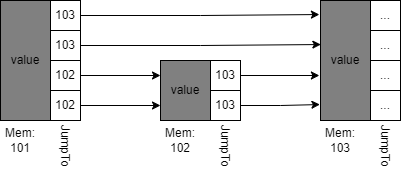
\includegraphics[width=9cm]{SkipList.drawio.png}
    \caption{Skip List Structure}
    \label{skip_list}
\end{figure}
\section{Coin Flip Functions}
For calculating the height of the list the implementation takes the approach of a coinflip in order to decide whether or not to promote a node up 1 level. Each time a coin is fliped and if it lands on heads it is promoted, that is unless it has reached max level.
\begin{minted}[frame=lines,framesep=2mm,baselinestretch=1.2,bgcolor=LightGray,
fontsize=\footnotesize,linenos,breaklines=true]{c++}
typedef enum coin_t{
    Heads, Tails
}coin_t;

SkipList::coin_t SkipList::flipCoin() {
    return rand() % 2 == 0 ? Heads : Tails;
}

int SkipList::generateLevel() {
    SkipList::coin_t coin = SkipList::Heads;
    int generatedLevel = 0;

    // ---------------------- If its Heads and we haven't reached Max Level add a level
    while (coin == SkipList::Heads && generatedLevel < MAX_LEVEL) {
        temporaryPromotions++;
        generatedLevel++;
        coin = flipCoin();
    }

    return generatedLevel;
}
\end{minted}
\section{Insertion Function}
In oderer for a node to be inserted into the list, the list first needs to be traversed in order for the insertion point to be found. Here a for-loop is traversed starting from the highest level down to the lowest, each time through a while loop skipping horizontally through nodes until a node with a larger value is found.

The function also keeps track of the last node used at each level in the update array. This is so that these can be updated once the node is inserted. 

It is important to note the steps are counted for both horizontal and vertical traversal. This means that the step counter is incremented both when the search moved down a level as well as when it jumps between nodes.
\begin{minted}[frame=lines,framesep=2mm,baselinestretch=1.2,bgcolor=LightGray,
fontsize=\footnotesize,linenos,breaklines=true]{c++}
SkipList::node_t* SkipList::searchInsert(int value, SkipList::node_t** update){
    SkipList::node_t* current = start_node;
    
    for (int i = highest_current_level; i >= 0; i--) {
        while (current->jumpTo[i] != nullptr && current->jumpTo[i]->value < value) {
            temporarySteps++;
            current = current->jumpTo[i];
        }
        temporarySteps++;
        update[i] = current;
    }
    
    return current;
}
\end{minted}
As stated before once the function is created the pointers of its jumTo list need to be updated as well as the preceding functions. This is where update is used. A for loop simply traverses the newly created node's jumpTo array updating the values of both its pointers and the jumpTo arrays held by update.
\begin{minted}[frame=lines,framesep=2mm,baselinestretch=1.2,bgcolor=LightGray,
fontsize=\footnotesize,linenos,breaklines=true]{c++}
void SkipList::create_And_insert(int value, int level, SkipList::node_t** update){
    node_t* newNode = new node_t(value, level);

    // -------------------- update the pointers for for the nodes to insert the node
    for (int i = 0; i < level; i++) {
        newNode->jumpTo[i] = update[i]->jumpTo[i];
        update[i]->jumpTo[i] = newNode;
    }
}
\end{minted}
The insertion first creates 2 pointers, one for the update list and the other pointing to the current location at which the new node should be placed. The function first makes use of the previously mentioned search function to get the insertion point. If the value being inserted is not a duplicate then a level is generated for the to-be-created node. If the generated level is higher than any other level in the skip list then the starting node or root node needs to be updated to point to it. 

It is after all this that the previously mentioned create\_And\_insert function is used to create and insert a node into its position in the list.
\begin{minted}[frame=lines,framesep=2mm,baselinestretch=1.2,bgcolor=LightGray,
fontsize=\footnotesize,linenos,breaklines=true]{c++}
void SkipList::insert(int value) {
    SkipList::node_t* update[MAX_LEVEL + 1];
    SkipList::node_t* current;

    current = searchInsert(value, update)->jumpTo[0];

    // -------------------- Check if value is a duplicate
    if (current == nullptr || current->value != value) {

        // -------------------- Randomly Generate the nodes Level
        int generatedLevel = generateLevel();
        
        // -------------------- If this is now the highest-level node we
        // -------------------- need to update both the starting node and the
        // -------------------- highest current Level
        if (generatedLevel > highest_current_level) {
            for (int i = highest_current_level; i < generatedLevel; i++) {
                update[i] = start_node;
            }
            highest_current_level = generatedLevel;
        }

        // -------------------- Insert and update the Linked list
        create_And_insert(value, generatedLevel, update);
    
    // -------------------- Key already in use
    }else{}
    updateStatistics();
}
\end{minted}


\section{Display Function}
The skip list display differs from that used for the previous tree data structures. Hence it will be covered in this section.

The function traverses in a top-down manner starting from the highest level in the skip list, printing the values for each level until a null node or the end of that level's list is reached

\begin{minted}[frame=lines,framesep=2mm,baselinestretch=1.2,bgcolor=LightGray,
fontsize=\footnotesize,linenos,breaklines=true]{c++}
void SkipList::printList() {
    std::cout << "==================SKIP LIST================== " << std::endl;
    for (int i = highest_current_level - 1; i >= 0; i--) {
        node_t* node = start_node->jumpTo[i];
        std::cout << "Level " << i << ": ";
        while (node != nullptr) {
            std::cout << node->value << " ";
            node = node->jumpTo[i];
        }
        std::cout << std::endl;
    }
}
\end{minted}

\chapter{Statistical Analysis}
\section{Explaining Statistics}
Height/Levels: The Height of a tree or the number of levels that were generated for the skip list.
Leaves: The number of leaf nodes in the tree.
\begin{table}[!htp]
    \centering 
    \begin{tabular}{|p{2cm}|p{5.5cm}||p{2cm}|p{5.5cm}|}
    \hline\multicolumn{4}{|c|}{Statistics}
    \\\hline
    \multicolumn{2}{|c||}{Steps} & \multicolumn{2}{|c|}{Rotations}
         \\\hline
         MIN& The minimum number of steps needed to reach the insertion point in both the AVL and skiplist&
         MIN& The minimum number of rotations/promotions needed after an insertion
         \\\hline
         MAX& The maximum number of steps needed to reach an insertion point&
         MAX& The maximum number of rotations/promotions needed to be made after an insertion
         \\\hline
         MEAN& The average number of steps needed to be made to reach an insertion point&
         MEAN& The average number of rotations/promotions needed after an insertion
         \\\hline
         STD& The standard deviation of the number of steps needed to reach an insertion point&
         STD& The standard deviation of the number of rotations/promotions needed after an insertion
         \\\hline
         MED& The median of the number of steps needed to reach an insertion point&
         MED& The median of the number of rotations/promotions needed after an insertion
         \\\hline
     \\\hline
    \end{tabular}
    \caption{Caption}
    \label{tab:my_label}
\end{table}

\section{Results Sample}
The below statistical output snippet contains the statistics both during the 5000 integer insertion, which was randomised using the Knuth shuffle, and the 1000 integer insertion after clearing the previous statistics record.
\begin{minted}[frame=lines,framesep=2mm,bgcolor = Arsenic,fontsize=\footnotesize, breaklines ]{console}
-------------------------------- 5000 Inserts 


==================== AVL Statistics =========================
HEIGHT: 15
LEAVES: 2140
Steps Statistics:
MIN: 1       MAX: 16      MEAN: 12.105  STD: 1.715   MED: 12      
Rotations Statistics:
MIN: 0       MAX: 1       MEAN: 0.463   STD: 0.499   MED: 0       
==================== RedBlack Statistics ====================
HEIGHT: 15
LEAVES: 2139
Steps Statistics:
MIN: 1       MAX: 16      MEAN: 12.125  STD: 1.736   MED: 12      
Rotations Statistics:
MIN: 0       MAX: 1       MEAN: 0.381   STD: 0.486   MED: 0       
==================== SkipList Statistics ====================
LEVELS: 14
Steps Statistics:
MIN: 1       MAX: 46      MEAN: 23.910  STD: 4.935   MED: 24      
Promotions Statistics:
MIN: 1       MAX: 14      MEAN: 2.037   STD: 1.455   MED: 2       


 -------------------------------- CLEAR 


==================== AVL Statistics =========================
No insertions where made
==================== RedBlack Statistics ====================
No insertions where made
==================== SkipList Statistics ====================
No insertions where made


 -------------------------------- 1000 Inserts 


==================== AVL Statistics =========================
HEIGHT: 15
LEAVES: 2539
Steps Statistics:
MIN: 7       MAX: 16      MEAN: 14.284  STD: 1.065   MED: 14      
Rotations Statistics:
MIN: 0       MAX: 1       MEAN: 0.465   STD: 0.499   MED: 0       
==================== RedBlack Statistics ====================
HEIGHT: 16
LEAVES: 2543
Steps Statistics:
MIN: 6       MAX: 17      MEAN: 14.560  STD: 1.192   MED: 15      
Rotations Statistics:
MIN: 0       MAX: 1       MEAN: 0.380   STD: 0.485   MED: 0       
==================== SkipList Statistics ====================
LEVELS: 14
Steps Statistics:
MIN: 17      MAX: 41      MEAN: 27.974  STD: 3.272   MED: 28      
Promotions Statistics:
MIN: 0       MAX: 11      MEAN: 1.891   STD: 1.464   MED: 1       
\end{minted}

One important thing to note is that the standard deviation for all 3 statistics was fairly low meaning that in general there were no major outliers and results where fairly close in value to the mean. The median also reflects this since it was usually around the same as the mean.

\section{Avl and RedBlack Trees}
First of all, both the Red Black Tree and Avl Tree hold similar statistics for all categories. Although in the sample above the RedBlack tree seems to have overall lower statistic values, this was not consistent as several reruns showed that depending on the values and input sequence either data structure could produce marginally better results over the other. The difference between results is not substantial enough to warrant the use of one over the other by itself.

Interestingly enough although both data structures resulted in the same height they usually resulted in different leaf counts showing that the different rotation and balancing implementations do affect the overall structure to sum marginally significant degree.

Another interesting point is that there is only ever need for at most 1 rotation. The statistic was consistent with the many reruns of the program. This means that balancing measures were always taken before the trees became vastly unbalanced. 

\section{Skip List}
The skip list data structure is harder to compare to the other data structures. Although it resembles some instances of a tree with the levels being comparable to the height, it is overall vastly different as a data structure than the previous two.

If the skip list's level count is to be considered a similar statistic to a tree's height then it can be said that the 3 datastructers on average generate similar heights. The skip list of course is overall less consistent due to the randomised nature but it usually falls in a similar range to the others. The skip list results show a marginal decrease in performance compared to the other data structures. The average steps are overall higher (in the case of the 2 chosen results by around twice as much).  The rotations and promotions aren't comparable to statistics since both are vastly different in terms of implementation and aims.

\section{Conclusion}
In order to reach a suitable conclusion it is best to take into account the difficulty of implementing any of the 3 data structures. Hence in the following analysis, the results will be in the view of comparing time/difficulty of implementation against the results.

The most simple implementation is that of the SkipList, under basic conditions in situations which don't require high performance this would be suitable. However, the inconsistency presented by the randomness of the promotions leaves much to be desired for heavier performance-related situations. This is because, unlike the other 2 data structures, the skip list doesn't always strive for the most optimal structure, and this can be seen especially in the mean number of steps. Even if the vertical steps were not to be counted, the results would still be similar.

The AVL tree would most likely be the option I would choose if I were in a situation where there was a need for an order-oriented data structure (meaning a situation where the values I am inserting have an order, not like for example the unordered\_set data structure). In terms of the difficulty of implementation, the AVL tree is not that much more difficult in terms of implementation compared to the skip list. It may be overall longer but the implementation doesn't require that complex thought to different cases that may arise. The performance is also worth the slightly more time-consuming implementation. 

This brings the discussion to the last data structure. The Red Black Tree although performing at the same level as the AVL tree, I found to have the overall highest difficulty in terms of implementation. The code reflects this as even the length is overall larger. The balancing implementation is much more complex inside the Red Black Tree requiring more cases to be taken into account. Since in both rotations, the maximum number was deemed to be 1 on average for the insertion, the added complexity of the Red Black Tree's insertion and red-red conflict handling may not be worth the effort. These results could be due to the specifically chosen implementation, and other implementations of Red-Black Trees could be simpler. 

In conclusion, the skip list would be a good option for a low-performance system while the AVL tree is better suited for higher performance due to its more reliable consistency. I would prefer the AVL tree when compared to the Red black tree due to the overall simpler implementation for the same marginal results.
\end{document}
